\documentclass[10pt]{article}
\usepackage[a4paper,margin=2cm]{geometry}
\setlength{\emergencystretch}{2em}
\usepackage{amsmath,amssymb,amsthm,mathtools}
\usepackage{booktabs,array}
\usepackage{graphicx}
\usepackage[dvipsnames]{xcolor}
\usepackage{tikz}
\usetikzlibrary{positioning,arrows.meta}
\usepackage{enumitem}
\usepackage[font=small]{caption}
\IfFileExists{microtype.sty}{\usepackage{microtype}}{}
% BibTeX backend keeps biblatex compatible with the current editor compiler.
\usepackage[backend=bibtex,style=numeric,sorting=none,giveninits=true,maxbibnames=99]{biblatex}
\addbibresource{references.bib}
\usepackage[colorlinks=true,linkcolor=MidnightBlue,citecolor=MidnightBlue,urlcolor=MidnightBlue]{hyperref}

% EDITORIAL SUPPORT: unchanged text is black; replacement/additional wording is red.
\newcommand{\rev}[1]{{\color{red}#1}}
% Preserve the existing editorial colouring in the generated bibliography.
\AtEveryBibitem{\ifkeyword{editorial-red}{\color{red}}{\color{black}}}
\DeclareFieldFormat{note}{\ifkeyword{editorial-version}{\rev{#1}}{#1}}
\DeclareFieldFormat{eprint:arxiv}{%
  \ifkeyword{editorial-version}
    {\rev{\mkbibacro{arXiv}\addcolon\space#1}}
    {\mkbibacro{arXiv}\addcolon\space#1}}
\newcommand{\MissingResult}{\ifmmode\text{\normalfont\color{red}\footnotesize[missing]}\else{\normalfont\color{red}\footnotesize[missing]}\fi}
\newcommand{\MissingAsset}[1]{\fbox{\begin{minipage}{0.92\linewidth}\centering\color{red}\small
\textbf{Source asset not supplied:} \texttt{\detokenize{#1}}.\\[3pt]
The original figure or table must be restored here; no replacement data have been generated.
\end{minipage}}}
\newif\ifmissingassets
\IfFileExists{numbers.tex}{}{\missingassetstrue}
\IfFileExists{fig_fill.pdf}{}{\missingassetstrue}
\IfFileExists{table_sens.tex}{}{\missingassetstrue}
\IfFileExists{table_pol.tex}{}{\missingassetstrue}
\IfFileExists{table_gcc.tex}{}{\missingassetstrue}
\IfFileExists{table_surge.tex}{}{\missingassetstrue}
\InputIfFileExists{numbers.tex}{}{\PackageWarning{editorial-review}{numbers.tex not supplied; numerical values remain missing}}
\providecommand{\AdaptN}{\MissingResult}
\providecommand{\AdaptRecMax}{\MissingResult}
\providecommand{\AdaptRecMedian}{\MissingResult}
\providecommand{\AdaptRecMin}{\MissingResult}
\providecommand{\Aval}{\MissingResult}
\providecommand{\CappedGapMax}{\MissingResult}
\providecommand{\DoverA}{\MissingResult}
\providecommand{\FillViolationMax}{\MissingResult}
\providecommand{\FullGapMedianSlack}{\MissingResult}
\providecommand{\FullShortMax}{\MissingResult}
\providecommand{\GCCProlongedFillLowA}{\MissingResult}
\providecommand{\GCCProlongedFillLowB}{\MissingResult}
\providecommand{\GCCProlongedGainHigh}{\MissingResult}
\providecommand{\GCCProlongedGainLow}{\MissingResult}
\providecommand{\GCCShortCount}{\MissingResult}
\providecommand{\GainRuleOneOFive}{\MissingResult}
\providecommand{\GainRuleOneTwentyFive}{\MissingResult}
\providecommand{\GainRuleTwoHundred}{\MissingResult}
\providecommand{\IntRatioMax}{\MissingResult}
\providecommand{\IntRatioMin}{\MissingResult}
\providecommand{\OldSwitchMax}{\MissingResult}
\providecommand{\QlearnDiff}{\MissingResult}
\providecommand{\RecOneOFive}{\MissingResult}
\providecommand{\RecOneTwentyFive}{\MissingResult}
\providecommand{\RecTwoHundred}{\MissingResult}
\providecommand{\RuleGapMax}{\MissingResult}
\providecommand{\RuleGapMedian}{\MissingResult}
\providecommand{\RuleWithinHalf}{\MissingResult}
\providecommand{\SensN}{\MissingResult}
\providecommand{\ShiftAdaptVsClassical}{\MissingResult}
\providecommand{\ShiftAdaptVsRule}{\MissingResult}
\providecommand{\SurgeEqual}{\MissingResult}
\providecommand{\SurgeFacPoint}{\MissingResult}
\providecommand{\SurgeFacRobust}{\MissingResult}
\providecommand{\SurgeN}{\MissingResult}
\providecommand{\SurgePricingMax}{\MissingResult}
\providecommand{\SurgePricingMin}{\MissingResult}
\providecommand{\SurgeRobustBestGain}{\MissingResult}
\providecommand{\SurgeRobustBetter}{\MissingResult}
\providecommand{\SurgeRobustWorse}{\MissingResult}
\providecommand{\SurgeRobustWorstLoss}{\MissingResult}
\providecommand{\ZeroGapMax}{\MissingResult}
\providecommand{\ZeroGapMedian}{\MissingResult}


\newtheorem{proposition}{Proposition}
\newtheorem{lemma}{Lemma}
\newtheorem{corollary}{Corollary}
\newcommand{\E}{\mathbb{E}}
\newcommand{\dl}{\delta}
\setlist{itemsep=1pt,topsep=2pt}

\title{\textbf{An Adaptive Stackelberg Model for Buffering Near-Capacity Refineries against Supply Uncertainty}}

\author{Zineb Chaatit$^{a}$, Yang Deng$^{a}$\thanks{Corresponding author: ydeng@aus.edu}\\[2pt]
\small $^{a}$Department of Industrial Engineering, American University of Sharjah, United Arab Emirates}
\date{}

\begin{document}
\maketitle
% Red replacements are controlled by \rev; missing-asset markers are independently red.
% FORMAT: removed forced negative space below the title.
\smallskip
\ifmissingassets
\noindent{\small\color{red}\textbf{Editorial preview.} Revised wording is red; unchanged wording is black. The supplied source omits numerical definitions, four tables and a figure. The marker \texttt{[missing]} denotes an unavailable value, not a numerical result.}\par\smallskip
\fi
\begin{abstract}\noindent
Export-oriented refineries in the Gulf Cooperation Council (GCC) \rev{can operate close to full capacity and depend on a limited number of maritime export routes}. Geopolitical supply shocks can stop a plant or block its export route for weeks to months, as in 2026, \rev{and can affect multiple facilities and export routes simultaneously}. We study such a refiner as a Stackelberg leader with \rev{finite production capacity subject to random outages}, selling to distributors (followers) that order in lots and fall back on a spot market. \rev{Followers' responses are approximated by an economic order quantity model with supply disruptions in which the leader's premium enters the incremental cost of spot sourcing.} \rev{Within this follower-response model, plant-specific disruptions leave participation thresholds unchanged, while region-wide shocks that raise spot prices can increase the premium buyers accept. Independently of this approximation, supplying all demand requires the production rate to be at least demand divided by availability, a necessary condition that is more restrictive than the classical $P>D$ when availability is below one.} \rev{We derive a closed-form protection-stock target and propose a capacity-aware buffer rule that distinguishes slack from critical or structurally short regimes.} Across \SensN{} simulated scenarios the rule is within \RuleGapMedian\% of \rev{the best tested grid policy at the median} and within 0.5\% in \RuleWithinHalf{} scenarios, while holding no buffer loses up to \ZeroGapMax\%. An adaptive leader that learns the disruption rates online and re-solves the game recovers a median \AdaptRecMedian\% of the value of knowing them \rev{and outperforms the tabular Q-learning implementation evaluated here}; under region-wide shocks, pricing against a cautious estimate of disruption severity \rev{reduces exposure to overpricing and buyer rejection in the tested scenarios}. \rev{Across four illustrative GCC-inspired disruption regimes}, the model shows that a refinery at 95\% utilisation is structurally short under every disruption regime except routine operations. \rev{All model data are synthetic.}
\end{abstract}
\noindent\textbf{Keywords:} capacity planning; geopolitical supply shocks; regional security disruptions; GCC refining; Stackelberg game; EOQ/EPQ; buffer stock; adaptive control.

%=====================================================================
\section{Introduction}
%=====================================================================
GCC refining is large, concentrated and export-oriented. \rev{Kuwait's Al-Zour refinery has a nominal refining capacity of 615,000 barrels per day \cite{kipic2023}, contributing to national capacity above 1.4 million b/d \cite{eiakuwait}. The Strait of Hormuz carried about 20 million b/d of oil in 2024 \cite{eiahormuz2025}.} This supply can be interrupted. \rev{Unplanned outages and planned turnarounds interrupt supply for varying durations; planned turnarounds can last from weeks to months \cite{afpm2023}.} In 2026, flows through Hormuz were disrupted from late February; global oil supply fell by 10.1 million b/d in March \cite{worldbank2026}, \rev{and the IEA reported that attacks and a lack of viable export outlets had shut more than 3 million b/d of regional refining capacity as storage filled \cite{iea2026march}.} Disruptions to Hormuz flows persisted through the second quarter of 2026 \cite{eia2026}. \rev{A blocked export route can prevent deliveries even when a plant remains operational. We use complete outages as a simplified representation of supply unavailability, while recognising that route closures and plant outages can have different effects on production and usable inventory.} Unlike a local breakdown, such regional security disruptions also tighten the spot market that buyers fall back on.

\rev{Near-capacity operation is observed in practice: US refineries, for comparison, operated at 95.5\% of operable capacity in the week ending 18 July 2025 \cite{eiautil2025}.} Near full capacity there is little slack to rebuild stock after an outage, so disruptions translate directly into lost supply.

\rev{Classical lot-sizing models do not jointly capture these features.} The economic production quantity (EPQ) model only requires the production rate to exceed demand ($P>D$), and as $P\to D$ it recommends ever longer production runs. \rev{Integrated vendor--buyer models \cite{lu1995} and Stackelberg lot-sizing models \cite{romeijn2012} address coordination and strategic interaction under reliable supply.} Disruption models \cite{parlar1991,berk1994,qi2009,snyder2016} capture unreliable supply but usually for a single decision maker, and studies of strategies against disruptions \cite{tomlin2006} do not model a capacity-limited leader whose buyers respond strategically.

We combine these elements in a model of a capacity-limited GCC refiner (leader) and its distributors or offtakers (followers). Our contributions are:
\begin{enumerate}[label=(\roman*),leftmargin=*]
\item \rev{We use the EOQ model with supply disruptions (EOQD) \cite{parlar1991} as a follower-response approximation in the Stackelberg framework. The leader's premium enters the incremental spot-sourcing cost. Within this response model, plant-specific disruptions leave participation thresholds unchanged (Lemma~\ref{lem:part}), although follower costs and leader sales can still change.}
\item We show that full supply requires $P\ge D/A$, where $A$ is plant availability (Proposition~\ref{prop:cap}), \rev{and derive an approximate protection-stock target used in a capacity-aware buffer rule (Section~\ref{sec:buffer}). The rule is benchmarked against the best tested grid policy in \SensN{} synthetic scenarios and illustrated using four GCC-inspired disruption regimes.}
\item We propose an adaptive leader that learns the disruption rates online and re-solves the game each period, and compare it with model-free Q-learning.
\end{enumerate}

%=====================================================================
\section{Related literature}
%=====================================================================
\textbf{Leader--follower lot sizing.} Integrated vendor--buyer models with equal shipments \cite{lu1995} and Stackelberg lot-sizing games \cite{romeijn2012} study coordination when each party optimises its own cost, under reliable supply. Capacity allocation games \cite{cachon1999} show that buyers inflate orders when a capacity-constrained supplier rations, but without lot sizing or disruptions.

\textbf{Inventory under supply disruptions.} Parlar and Berkin \cite{parlar1991} introduced the EOQ model with a randomly available supplier, later revisited by Berk and Arreola-Risa \cite{berk1994}; Qi et al.\ \cite{qi2009} add retailer disruptions, Snyder \cite{snyder2014} gives a tight approximation, and Snyder et al.\ \cite{snyder2016} review the area. Tomlin \cite{tomlin2006} compares inventory, sourcing and contingent rerouting against disruptions. Leader--follower models with disruption risk have studied resilience investment and cost-sharing contracts \cite{luo2024}, and supplier reliability with a spot market has been studied with competing suppliers \cite{gumus2012}.

\textbf{Learning under unreliable supply.} Tomlin \cite{tomlin2009} studies a buyer that learns supplier reliability; learning in Stackelberg settings has been studied with reinforcement learning \cite{brero2024}.

\rev{\textbf{Positioning.} We study the joint role of (a) EOQD-based follower responses, (b) a leader with a finite production rate close to demand, and (c) a leader buffer policy that accounts for stock replenishment between outages, together with online learning of the disruption rates.}

%=====================================================================
\section{Model}
%=====================================================================
\textbf{Setting and notation.} Time is in days; the leader decides once a month. Followers $i=1,\dots,n$ face constant demand $d_i$ (total $D=\sum_id_i$), ordering cost $K_i$ and holding cost $h_i$. Prices are measured relative to a fluctuating benchmark $m_t$: the leader charges $m_t+\dl$, where the premium $\dl\in[\dl_{\min},\dl_{\max}]$ is bounded; followers resell at margin $g$ and can buy spot at premium $\theta_i$ plus a per-unit ordering-and-holding cost $\kappa_i=\sqrt{2K_ih_i/d_i}$.

The leader produces at rate $P$ when its plant is up. Up and down periods are exponential with rates $\lambda$ (disruption) and $\mu$ (recovery), so availability is $A=\mu/(\lambda+\mu)$. When up, the leader runs production at rate $P$ until stock reaches $S=B+\max_iQ_i$ (buffer $B$ plus cycle stock). Each run is an EPQ-type lot produced at finite rate, \rev{with stock building at the fluid rate $P-D$ when all nominal demand is served}; a setup costs $K_L$ and holding costs $h_L$ per unit-day. Its margin is $M=m_t+\dl-c$. Utilisation is $\rho=D/P$.

% AUTHOR CHECK 1: Specify the leader objective and the premium/buffer optimisation procedure.
% AUTHOR CHECK 2: Clarify D when followers leave, and the recent-purchase rationing window/tie rule.
\textbf{Game and timing.} Each month (Fig.~\ref{fig:timing}) the leader commits to $(\dl,B)$ (Stage 1). Each follower decides whether to buy from the leader and chooses its lot size $Q_i$ (Stage 2). Followers use zero-inventory ordering; demand they cannot cover from their own stock is bought spot. If requests exceed the leader's stock, stock is rationed in proportion to recent purchases.

\begin{figure}[t]
\centering
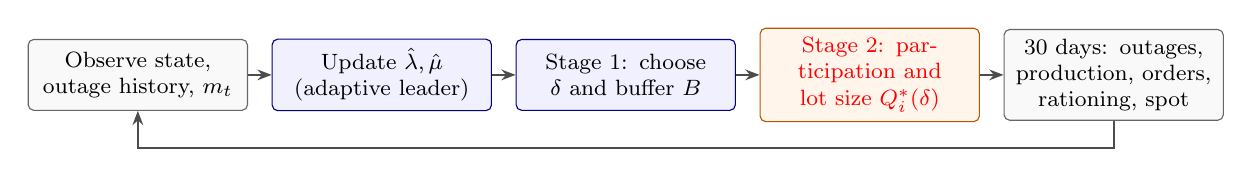
\begin{tikzpicture}[node distance=3mm,
 b/.style={draw=black!60,rounded corners=2pt,fill=gray!5,align=center,font=\footnotesize,minimum height=9mm,text width=2.55cm},
 l/.style={b,fill=blue!6,draw=blue!50!black}, f/.style={b,fill=orange!8,draw=orange!70!black},
 a/.style={-{Stealth[length=1.8mm]},thick,black!70}]
\node[b] (o) {Observe state, outage history, $m_t$};
\node[l,right=of o] (e) {Update $\hat\lambda,\hat\mu$ (adaptive leader)};
\node[l,right=of e] (s1) {Stage 1: choose $\dl$ and buffer $B$};
\node[f,right=of s1] (s2) {\rev{Stage 2: participation and lot size $Q_i^*(\dl)$}};
\node[b,right=of s2] (op) {30 days: outages, production, orders, rationing, spot};
\draw[a] (o)--(e); \draw[a] (e)--(s1); \draw[a] (s1)--(s2); \draw[a] (s2)--(op);
\draw[a] (op.south) -- ++(0,-0.35) -| (o.south);
\end{tikzpicture}
\caption{Monthly sequence. Blue: leader; orange: followers.}
\label{fig:timing}
\end{figure}

\rev{\textbf{Follower-response approximation.} The analytical response model assumes that a follower's order is filled immediately when the supplier is up, and cannot be filled while it is down. It abstracts from the leader's finite stock, buffer-supported deliveries and rationing. The responses below therefore approximate, rather than establish best responses to, the full operational simulation. Let} $\psi_i(Q)=\frac{\lambda}{\lambda+\mu}\big(1-e^{-(\lambda+\mu)Q/d_i}\big)$ be the probability that the leader is down when a lot runs out, given that it was up when the lot was ordered. By the renewal--reward argument of the EOQD model \cite{parlar1991,snyder2019}, the expected cost per day of lot size $Q$ with shortage cost $s$ is
\begin{equation}\label{eq:G}
G_i(Q;s)=\frac{K_i+h_iQ^2/(2d_i)+s\,d_i\psi_i(Q)/\mu}{Q/d_i+\psi_i(Q)/\mu},
\end{equation}
\rev{and $\beta_i(Q)=\frac{Q/d_i}{Q/d_i+\psi_i(Q)/\mu}$ is the leader-supplied share in this response approximation.} To capture region-wide shocks, spot purchases made while the leader is down cost an extra $\xi\ge0$ (a surge), and $\xi=0$ describes a plant-specific outage. \rev{Writing the incremental per-unit spot-sourcing cost during an outage as $s_i(\dl)=\theta_i+\kappa_i+\xi-\dl$}, the benchmark cancels and the follower's profit per day is
\begin{equation}\label{eq:follower}
\Pi_i(Q\mid\dl)=(g-\dl)d_i-G_i\big(Q;\,s_i(\dl)\big),
\end{equation}
against an outside option of $\big(g-\theta_i-\kappa_i-(1-A)\xi\big)d_i$ (buy everything spot, paying the surge during the share $1-A$ of time the region is disrupted). \rev{Within these delivery assumptions, the follower problem has the EOQD form, with an incremental shortage cost that depends on the leader's premium.} As $\lambda\to0$, $\psi_i\to0$ and \eqref{eq:G} reduces to the EOQ cost.

%=====================================================================
\section{Analysis}
%=====================================================================
\begin{lemma}[Participation]\label{lem:part}
\rev{Within the EOQD response model, and with indifference resolved in favour of participation, follower $i$ buys from the leader if and only if $\dl\le\bar\dl_i$, where}
\[
\theta_i+\xi\Big(1-\frac{A}{\beta_i(Q_i^{\text{EOQ}})}\Big)\ \le\ \bar\dl_i\ \le\ \theta_i+\xi(1-A).
\]
For plant-specific outages ($\xi=0$), $\bar\dl_i=\theta_i$ for all $\lambda,\mu$.
\end{lemma}
\begin{proof}
By the arithmetic--geometric mean inequality, $K_i+h_iQ^2/(2d_i)\ge\kappa_iQ$, with equality at the EOQ lot size. Hence $G_i(Q;s)\ge\kappa_id_i-(\kappa_i-s)d_i(1-\beta_i(Q))$, and with $s=s_i(\dl)$ the gain over the outside option satisfies
\[
\Pi_i(Q\mid\dl)-\big(g-\theta_i-\kappa_i-(1-A)\xi\big)d_i\ \le\ (\theta_i-\dl)\,d_i\,\beta_i(Q)+\xi\,d_i\big(\beta_i(Q)-A\big),
\]
\rev{with equality at the EOQ lot size. The gain optimised over $Q$ is decreasing in $\dl$, because each fixed-$Q$ gain has slope $-d_i\beta_i(Q)<0$. At EOQ the right side is non-negative exactly when} $\dl\le\theta_i+\xi(1-A/\beta_i)$, which gives the lower bound. If $\dl>\theta_i+\xi(1-A)$, the right side is below $\xi d_iA(\beta_i-1)\le0$ for every $Q$, which gives the upper bound. With $\xi=0$ both bounds equal $\theta_i$.
\end{proof}
\noindent \rev{Within the EOQD response model, plant-specific outages leave participation thresholds unchanged. This does not imply that follower profits are unchanged; the leader additionally loses sales.} \rev{Within the same response model, region-wide shocks can increase the participation threshold} because a follower's own stock covers part of each outage ($\beta_i>A$), relying on the refiner exposes it to the surge less than buying spot, so it accepts a premium up to $\xi(1-A)$ higher. The threshold then depends on $\lambda$ and $\mu$, so pricing requires knowing how severe disruptions are. \rev{In the reported synthetic base case, an integrated chain that also counts the leader's lost margin would order lots} \IntRatioMin--\IntRatioMax{} times larger. Moreover, because $G_i$ is linear in $s$ with slope $d_i(1-\beta_i(Q))$, which decreases in $Q$, \rev{Topkis's theorem implies that the smallest and largest optimal lot-size selections are non-increasing in $\dl$ for participating followers in this response model: a higher premium can reduce their inventory protection.}

\begin{proposition}[Capacity under disruptions]\label{prop:cap}
Under any leader policy, the long-run share of demand supplied by the leader is at most $\min(1,A/\rho)$. Supplying all demand therefore requires $P\ge D/A$.
\end{proposition}
\begin{proof}
Over $T$ days, shipments cannot exceed initial stock plus production, which is at most $P$ times the number of up days. Dividing by $DT$ and letting $T\to\infty$, the share of up days tends to $A$ and initial stock$/DT\to0$.
\end{proof}
\noindent \rev{We call $\rho>A$ \emph{structural shortage}: mean available production is below nominal demand, so long-run supply cannot reach that demand. The equality $\rho=A$ is the critical boundary; the upper-bound argument alone does not exclude a supply share of one there.} With $A=\Aval$ in our base case, the threshold is $P=\DoverA$, so a plant at 95\% utilisation is structurally short even though the classical EPQ condition $P>D$ holds.

% AUTHOR CHECK 3: In the critical/short regime, does Z* denote S or B? If B=Z*, then S=Z*+max Q. Match the code and tables.
\subsection{Capacity-aware buffer rule}\label{sec:buffer}
Let $Z$ be the protection stock in the system when an outage starts. An outage of length $\tau\sim\text{Exp}(\mu)$ loses approximately $D(\tau-Z/D)^+$ sales, and $\E[(\tau-b)^+]=e^{-\mu b}/\mu$. Outages start at rate $\lambda A$ per day. \rev{For $M>0$, minimising the approximate holding-cost and expected-lost-margin objective,} $h_LZ+\lambda AM\frac{D}{\mu}e^{-\mu Z/D}$, which is convex in $Z$, gives
\begin{equation}\label{eq:Z}
\begin{aligned}
Z^*&=\frac{D}{\mu}\max\Big\{0,\ \ln\frac{\lambda AM}{h_L}\Big\},\\
B_{\text{target}}&=\Big(Z^*-\tfrac12\textstyle\sum_iQ_i^*-\tfrac12\max_iQ_i^*\Big)^{+}.
\end{aligned}
\end{equation}
\rev{For $M\le0$, the minimiser of this surrogate is $Z^*=0$. The subtracted terms approximate stock already held by followers and in the leader's cycle stock; they do not establish its distribution at outage onset.} \rev{Under the fluid approximation with all followers participating, stock refills at rate $P-D$ during an up period, whose mean duration is $1/\lambda$. Thus $B_{\text{cap}}=(P-D)/\lambda$ is a mean potential refill volume during one up period, rather than an upper bound on sustainable inventory.} \rev{The proposed heuristic is:}
\begin{itemize}[leftmargin=*]
\item if $\rho<A$ (slack): produce up to $B_{\text{target}}+\max_iQ_i^*$. $B_{\text{cap}}<B_{\text{target}}$ only signals that the buffer will often be below target after an outage; producing at full rate instead would let stock grow without bound;
\item \rev{if $\rho\ge A$ (critical or structurally short): the heuristic omits the stock corrections and uses $Z^*$ as its protection target. When $\rho>A$, the strict mean-capacity deficit limits replenishment. The finite target limits accumulation during unusually long up periods.}
\end{itemize}
\rev{The rule links buffering to production slack. Mean supply slack $AP-D$ vanishes as $\rho$ approaches $A$ from below, whereas $B_{\text{cap}}$ does not: for fixed $D$, its limit is $D/\mu$. When $\rho>A$, inventory cannot remove the mean-capacity deficit; capacity, availability or nominal demand must change to remove that deficit.}

%=====================================================================
% AUTHOR CHECK 4: Confirm exact transition/exposure observations, cumulative statistics, gamma prior shapes/rates and discounting of both counts and exposure. Daily endpoint observations alone require a different likelihood.
\section{Adaptive leader}
%=====================================================================
In practice $\lambda$ and $\mu$ are unknown and may change. The adaptive leader keeps the Stackelberg structure and replaces them by estimates. \rev{For the undiscounted estimator, let $U$ and $W$ denote cumulative observed up- and down-time, and $N^{\downarrow}$ and $N^{\uparrow}$ cumulative outage and recovery counts. The point estimates are} $\hat\lambda=(a_0+N^{\downarrow})/(b_0+U)$ and $\hat\mu=(a_1+N^{\uparrow})/(b_1+W)$. \rev{With exact transition counts and exposure times and no discounting, these are posterior means under gamma priors parameterised by shape and rate. They approach the corresponding maximum-likelihood estimates as exposure accumulates.} It then predicts the followers' Stage~2 responses with $(\hat\lambda,\hat\mu)$, chooses $\dl$, and applies the buffer rule with $(\hat\lambda,\hat\mu,m_t)$. Its prior is deliberately optimistic (outages every 365 days lasting 7 days). Because followers' thresholds rise with disruption severity when $\xi>0$, \rev{the leader uses a cautious pricing heuristic based on} the 10\% posterior quantile of $\lambda$ and the 90\% quantile of $\mu$ (gamma posteriors). The buffer uses the point estimates. \rev{To track changes, both the past transition counts and the corresponding exposure times for $\lambda$ can be discounted by a factor $f<1$ per month. Such discounted updates are an adaptation heuristic rather than ordinary posterior updating for a stationary rate.}

%=====================================================================
% AUTHOR CHECK 5: Confirm evaluation duration/warm-up, matched shock paths, seed-level paired standard errors and definitions/denominators for every gap and recovery measure.
% AUTHOR CHECK 6: Supply the Q-learning states, actions, reward, discounting, learning/exploration schedules, training/evaluation seeds and exploration-free evaluation protocol.
\section{Numerical study}
%=====================================================================
\textbf{Design.} \rev{Base case (synthetic):} $d=(50,30,20)$ units/day, $K_i=400$, $h_i=0.04$, $\theta=(6.5,4.5,2.5)$, $g=10$, $c=20$, $\bar m=75$ with AR(1) benchmark ($\phi=0.8$, $\sigma=4$), $h_L=0.02$, $K_L=2000$, $\lambda=1/180$, $\mu=1/14$, premium grid $\{0,1,\dots,6\}$. The plant is simulated daily; \rev{results are averaged over 30 years after a two-year warm-up, using 10 random seeds.} Policies share seeds (common random numbers), and differences are reported as paired means $\pm$ standard error. The sensitivity analysis crosses mean time between outages $\{90,180,365\}$ days, mean outage length $\{7,14,28\}$ days, utilisation $\rho\in\{0.50,0.80,0.90,0.95\}$ and $h_L\in\{0.01,0.02,0.05\}$, giving \SensN{} scenarios (20 years, 6 seeds each). In each, the rule is compared with the best of a buffer grid $B\in\{0,0.5,1,2,3,4\}\times D/\mu$ plus full-rate production.

\textbf{Capacity bound.} \rev{Fig.~\ref{fig:fill} illustrates Proposition~\ref{prop:cap}: once utilisation exceeds availability, the long-run supplied share cannot exceed $A/\rho$. With a large buffer, the reported simulation approaches this bound.}

\begin{figure}[t]
\centering
\IfFileExists{fig_fill.pdf}{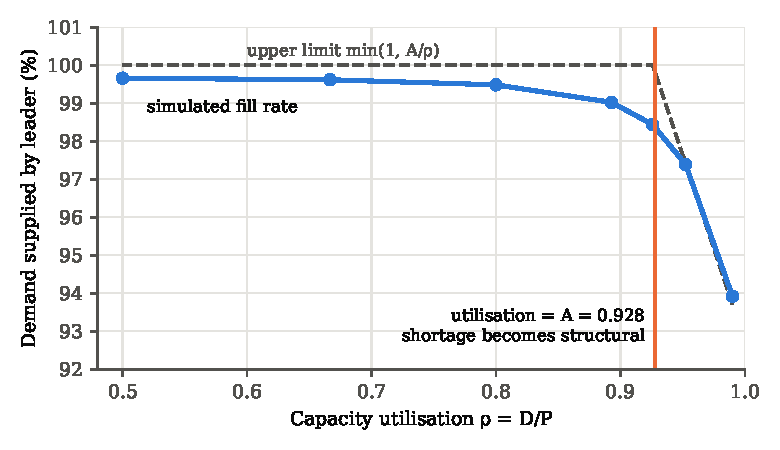
\includegraphics[width=0.62\textwidth]{fig_fill.pdf}}{\MissingAsset{fig_fill.pdf}}
\caption{Share of demand supplied by the leader (large buffer) versus utilisation, base case.}
\label{fig:fill}
\end{figure}

\rev{\textbf{Buffer-rule performance.}} Table~\ref{tab:sens} summarises the gap to the best grid buffer. The rule's median gap is \RuleGapMedian\%, its maximum \RuleGapMax\%, and it is within 0.5\% in \RuleWithinHalf{} of \SensN{} scenarios. Never holding a buffer loses \ZeroGapMedian\% at the median and up to \ZeroGapMax\%. Always producing at full rate loses \FullGapMedianSlack\% at the median when the plant has slack, because stock accumulates; \rev{in the structurally short cases considered, its reported profit is close to the best tested grid policy} \rev{but full-rate production still loses up to \FullShortMax\%} when outages are long and holding is costly, which the finite target $Z^*$ avoids. \rev{Two tested variants motivate placing the heuristic switch at $\rho=A$:} capping the target at $B_{\text{cap}}$ (maximum gap \CappedGapMax\%) and switching to full rate whenever $B_{\text{cap}}<B_{\text{target}}$ (up to \OldSwitchMax\%). Measured against each run's realised uptime, the supplied share never exceeds the bound of Proposition~\ref{prop:cap} by more than \FillViolationMax{} percentage points (the effect of initial stock).

\begin{table}[t]
\centering\small
\caption{Profit gap to the best grid buffer (\%), \SensN{} scenarios. \rev{``Short'' groups critical or structurally short scenarios with $\rho\ge A$.}}
\label{tab:sens}
\IfFileExists{table_sens.tex}{\begin{tabular}{@{}lccccccc@{}}
\toprule
 & & \multicolumn{2}{c}{Rule} & \multicolumn{2}{c}{No buffer} & \multicolumn{2}{c}{Full rate} \\
\cmidrule(lr){3-4}\cmidrule(lr){5-6}\cmidrule(lr){7-8}
Utilisation $\rho$ & Short & median & max & median & max & median & max \\
\midrule
0.50 & 0/27 & 0.01 & 0.41 & 1.17 & 7.46 & $>$100 & $>$100 \\
0.80 & 3/27 & 0.14 & 0.60 & 1.17 & 8.49 & 22.48 & 85.63 \\
0.90 & 9/27 & 0.22 & 0.72 & 1.60 & 4.81 & 3.57 & 33.08 \\
0.95 & 18/27 & 0.07 & 0.53 & 0.70 & 2.33 & 0.00 & 11.36 \\
\midrule
All & 30/108 & 0.13 & 0.72 & 1.01 & 8.49 & 10.24 & $>$100 \\
\bottomrule
\end{tabular}
}{\MissingAsset{table_sens.tex}}
\end{table}

\textbf{Policies.} Table~\ref{tab:pol} compares, in the base case, a classical leader (premium chosen as if $\lambda=0$, no buffer), the rule with the true rates, and the adaptive leader. The rule gains \GainRuleTwoHundred, \GainRuleOneTwentyFive{} and \GainRuleOneOFive{} per year over the classical leader at $\rho=0.50,0.80,0.95$. The adaptive leader, \rev{starting from an optimistic prior}, recovers \RecTwoHundred\%, \RecOneTwentyFive\% and \RecOneOFive\% of that gain. Across the \AdaptN{} sensitivity scenarios where it was run, it recovers \AdaptRecMin--\AdaptRecMax\% (median \AdaptRecMedian\%). When the outage frequency doubles without notice in month 120 ($\rho=0.80$), the adaptive leader earns \ShiftAdaptVsRule{} per year relative to the rule tuned to the old rates and \ShiftAdaptVsClassical{} relative to the classical leader. A tabular Q-learning leader trained for 800 simulated years earns \QlearnDiff{} per year relative to the adaptive leader at $\rho=0.95$.

\begin{table}[t]
\centering\small
\caption{Base-case policies: leader profit per year, share of demand supplied, and gain over the classical leader (paired mean $\pm$ s.e.).}
\label{tab:pol}
\IfFileExists{table_pol.tex}{\begin{tabular}{@{}llrcr@{}}
\toprule
$\rho$ & Policy & Leader profit/yr & Supplied & Gain vs classical \\
\midrule
0.50 & Classical & 1{,}949{,}373 & 98.00\% & -- \\
 & Rule (true rates) & 1{,}972{,}649 & 99.55\% & $+23{,}275\pm3{,}152$ \\
 & Adaptive & 1{,}968{,}362 & 99.22\% & $+18{,}989\pm2{,}529$ \\
\addlinespace
0.80 & Classical & 1{,}965{,}109 & 97.54\% & -- \\
 & Rule (true rates) & 1{,}988{,}543 & 99.21\% & $+23{,}434\pm2{,}942$ \\
 & Adaptive & 1{,}984{,}731 & 98.84\% & $+19{,}622\pm3{,}026$ \\
\addlinespace
0.95 & Classical & 1{,}963{,}762 & 96.38\% & -- \\
 & Rule (true rates) & 1{,}988{,}959 & 97.72\% & $+25{,}197\pm2{,}249$ \\
 & Adaptive & 1{,}982{,}767 & 97.35\% & $+19{,}005\pm1{,}714$ \\
\bottomrule
\end{tabular}
}{\MissingAsset{table_pol.tex}}
\end{table}

% AUTHOR CHECK 7: The listed factorial grid gives 108 scenarios; the four regime availabilities imply 6 of 12 strictly short combinations. Verify these against numbers.tex; no missing numerical result has been filled in here.
\textbf{GCC disruption regimes.} \rev{Motivated by the documented events, we specify four illustrative GCC-inspired regimes:} \emph{routine} operations (an outage every 365 days lasting 7 days on average), \emph{facility outages} \rev{(every 180 days, lasting 14 days on average)}, \emph{prolonged disruption} (every 90 days, 28 days) and \emph{export-route closure} (one closure a year lasting 60 days, as when an export route is blocked for months). Table~\ref{tab:gcc} reports availability, whether the refinery is structurally short, and the gains of the rule and the adaptive leader over the classical leader at utilisations of 0.80, 0.90 and 0.95. \GCCShortCount{} of the 12 combinations are structurally short; at 95\% utilisation every regime except routine operations is. In those cases no buffer restores full supply. The value of buffering also falls with utilisation: under prolonged disruption the rule raises the supplied share from \GCCProlongedFillLowA\% to \GCCProlongedFillLowB\% and gains about \GCCProlongedGainLow{} thousand per year at 80\% utilisation, but only \GCCProlongedGainHigh{} thousand at 95\%, because a plant with almost no slack cannot rebuild stock between outages. Under routine operations the rule holds no buffer, so it coincides with the classical leader.

\begin{table}[t]
\centering\small
\caption{\rev{Illustrative GCC-inspired disruption regimes} ($h_L=0.02$; 20 years, 6 seeds). Gains are leader profit per year over the classical leader, in thousands (paired mean $\pm$ s.e.).}
\label{tab:gcc}
\IfFileExists{table_gcc.tex}{\begin{tabular}{@{}lccccrr@{}}
\toprule
Regime (days between, length) & $A$ & $\rho$ & Short & Supplied: classical $\to$ rule & Rule gain & Adaptive gain \\
\midrule
Routine (365, 7) & 0.981 & 0.80 & no & 99.7\% $\to$ 99.7\% & $+0.0\pm0.0$ & $-0.1\pm0.8$ \\
 &  & 0.90 & no & 99.6\% $\to$ 99.6\% & $+0.0\pm0.0$ & $+1.2\pm0.7$ \\
 &  & 0.95 & no & 99.5\% $\to$ 99.5\% & $+0.0\pm0.0$ & $+0.6\pm1.1$ \\
\addlinespace
Facility outages (180, 14) & 0.928 & 0.80 & no & 97.0\% $\to$ 98.8\% & $+26.0\pm3.4$ & $+23.0\pm3.9$ \\
 &  & 0.90 & no & 96.5\% $\to$ 98.3\% & $+33.3\pm4.8$ & $+26.1\pm3.4$ \\
 &  & 0.95 & yes & 95.8\% $\to$ 97.4\% & $+30.9\pm4.0$ & $+20.9\pm2.5$ \\
\addlinespace
Prolonged disruption (90, 28) & 0.763 & 0.80 & yes & 88.3\% $\to$ 96.2\% & $+144.6\pm9.4$ & $+117.9\pm9.1$ \\
 &  & 0.90 & yes & 85.5\% $\to$ 87.6\% & $+42.2\pm3.3$ & $+42.0\pm3.0$ \\
 &  & 0.95 & yes & 82.8\% $\to$ 83.0\% & $+4.6\pm1.3$ & $+4.6\pm1.3$ \\
\addlinespace
Export-route closure (365, 60) & 0.859 & 0.80 & no & 90.4\% $\to$ 96.5\% & $+81.7\pm17.4$ & $+55.2\pm7.9$ \\
 &  & 0.90 & yes & 90.0\% $\to$ 95.1\% & $+77.6\pm12.7$ & $+50.5\pm4.9$ \\
 &  & 0.95 & yes & 89.4\% $\to$ 91.8\% & $+44.7\pm3.3$ & $+35.3\pm4.7$ \\
\bottomrule
\end{tabular}
}{\MissingAsset{table_gcc.tex}}
\end{table}

\textbf{Region-wide shocks.} Table~\ref{tab:surge} repeats the regimes at 90\% utilisation with a spot surge $\xi\in\{0,5,10\}$ during outages. As Lemma~\ref{lem:part} predicts, the smallest buyer's acceptable premium rises with $\xi$, most in the prolonged-disruption regime, where the refiner can raise its premium from 2 to 3 on our integer grid without losing any buyer; that pricing effect alone is worth \SurgePricingMin--\SurgePricingMax{} thousand per year across utilisations. Because thresholds now depend on disruption severity, an adaptive leader that prices at its point estimates sometimes believes a buyer will accept a price it in fact rejects, and loses that buyer for a month. In the facility-outage regime with $\xi=10$ its gain over the classical leader is \SurgeFacPoint{} thousand, against \SurgeFacRobust{} with cautious pricing. \rev{Cautious pricing reduces losses from rejected offers in the reported scenarios:} across the \SurgeN{} surge scenarios it is better in \SurgeRobustBetter{} (by up to \SurgeRobustBestGain{} thousand per year, \rev{with lower reported variation}), identical in \SurgeEqual{}, and worse in \SurgeRobustWorse{}, by at most \SurgeRobustWorstLoss{} thousand, where a higher price would have been safe.

\begin{table}[t]
\centering\small
\caption{Region-wide shocks at 90\% utilisation: smallest buyer's acceptable premium, the refiner's chosen premium, and gains over the classical leader in thousands per year (paired mean $\pm$ s.e.). ``Cautious'' prices at the 10\%/90\% posterior quantiles.}
\label{tab:surge}
\IfFileExists{table_surge.tex}{\begin{tabular}{@{}lcccrrr@{}}
\toprule
 & & Smallest buyer's & Premium & Rule & \multicolumn{2}{c}{Adaptive gain} \\ \cmidrule(lr){6-7}
Regime & Surge $\xi$ & limit $\bar\delta_3$ & $\delta^*$ & gain & cautious & point est. \\
\midrule
Routine & 0 & 2.50 & 2 & $+0.0\pm0.0$ & $+1.2\pm0.7$ & $+1.2\pm0.7$ \\
 & 5 & 2.57 & 2 & $+0.0\pm0.0$ & $+0.5\pm0.3$ & $+0.5\pm0.3$ \\
 & 10 & 2.65 & 2 & $+0.0\pm0.0$ & $-0.0\pm0.7$ & $-0.0\pm0.7$ \\
\addlinespace
Facility outages & 0 & 2.50 & 2 & $+33.3\pm4.8$ & $+26.1\pm3.4$ & $+26.1\pm3.4$ \\
 & 5 & 2.73 & 2 & $+27.6\pm4.3$ & $+22.5\pm2.7$ & $+22.5\pm2.7$ \\
 & 10 & 2.97 & 2 & $+25.6\pm3.1$ & $+18.7\pm2.3$ & $-15.7\pm30.4$ \\
\addlinespace
Prolonged disruption & 0 & 2.50 & 2 & $+42.2\pm3.3$ & $+42.0\pm3.0$ & $+42.0\pm3.0$ \\
 & 5 & 3.12 & 3 & $+51.8\pm2.2$ & $+21.6\pm2.3$ & $+34.4\pm4.6$ \\
 & 10 & 3.82 & 3 & $+41.0\pm2.0$ & $+38.3\pm2.5$ & $+40.7\pm2.1$ \\
\addlinespace
Export-route closure & 0 & 2.50 & 2 & $+77.6\pm12.7$ & $+50.5\pm4.9$ & $+50.5\pm4.9$ \\
 & 5 & 2.69 & 2 & $+69.8\pm11.7$ & $+43.2\pm4.9$ & $+43.2\pm4.9$ \\
 & 10 & 2.90 & 2 & $+64.0\pm12.2$ & $+39.3\pm5.7$ & $+25.8\pm9.2$ \\
\bottomrule
\end{tabular}
}{\MissingAsset{table_surge.tex}}
\end{table}

%=====================================================================
\section{Managerial insights and limitations}
%=====================================================================
\begin{itemize}[leftmargin=*]
\item \rev{\textbf{Account for availability in capacity planning.} With disruptions, $P\ge D/A$ is a necessary condition for full nominal supply. At 95\% utilisation, every illustrative regime considered except routine operations has a strict mean-capacity deficit, which no stocking policy can eliminate.}
\item \rev{\textbf{Replenishment slack limits sustained inventory protection.} Mean production slack $AP-D$ vanishes at $\rho=A$, while $(P-D)/\lambda$ measures potential refill volume during an up period. Above the threshold, buffering can mitigate individual outages but cannot eliminate the mean-capacity deficit.}
\item \rev{\textbf{Participation does not imply full inventory protection.} In the EOQD response model with plant-specific outages, participation thresholds remain unchanged, but both follower costs and the refiner's lost sales can change. The reported integrated benchmark suggests that decentralised inventory protection can be insufficient from the chain's perspective.}
\item \rev{\textbf{Regional spot-market tightening can increase acceptable premiums.} In the response model, an outage-related spot surge can increase the premium buyers accept. Pricing near that threshold is sensitive to disruption-rate estimates. The cautious pricing heuristic reduces rejection losses in some tested scenarios, while foregoing revenue in others.}
\item \rev{\textbf{Learning disruption rates can support adaptation.} In the reported scenarios, estimating two disruption parameters within the specified model recovers much of the gain obtained with known rates and responds to the simulated regime change. Its comparison with Q-learning concerns the tabular implementation evaluated here.}
\end{itemize}
\textbf{Limitations.} \rev{Model data are synthetic and the regimes are illustrative; outages are exponential and complete,} whereas bypass routes (e.g.\ pipelines to the Red Sea and Gulf of Oman) make some closures partial; \rev{followers know $\lambda,\mu$, while their EOQD response approximation excludes the leader's buffer and rationing; consequently, an equilibrium of the coupled finite-stock system has not been established;} the surge $\xi$ is constant and known; the buffer rule is approximate. Natural extensions are surges that vary over time, followers that learn, partial outages and a maximum production-run length.

\paragraph{Declaration of generative AI use.} \textit{[To be completed by the authors according to the venue's policy: describe which parts of the derivations, code and text were prepared with AI assistance and confirm that the authors reviewed and take responsibility for the content.]}

\begingroup
\renewcommand*{\bibfont}{\small}
\setlength{\bibitemsep}{0pt}
\printbibliography[title={References}]
\endgroup
\end{document}
